\appendix

\chapter{Các tham số}
 \label{Appendix1}

\section{Sự thay đổi của $\sqrt{\beta}$ và $\sqrt{1-\beta}$}

%Praesent in sapien. Lorem ipsum dolor sit amet, consectetuer 
%adipiscing elit. Duis fringilla tristique neque. Sed interdum 
%libero ut metus. Pellentesque placerat.

Quá trình diffusion có thể được hiểu là một chuỗi các bước nhỏ, trong đó mỗi bước sẽ thay đổi trạng thái của hệ thống theo một cách ngẫu nhiên. Các hệ số quan trọng trong quá trình này bao gồm:
\begin{itemize}
	\item $\sqrt{\beta_t}$: Biểu diễn sự thay đổi trong mỗi bước $t$, đặc trưng cho cường độ của nhiễu trong từng bước.
	\item $\sqrt{1 - \beta}$: Biểu thị xác suất hệ thống giữ lại trạng thái trước đó mà không bị ảnh hưởng bởi nhiễu.
\end{itemize}

\begin{wrapfigure}{l}{0.3\textwidth}
	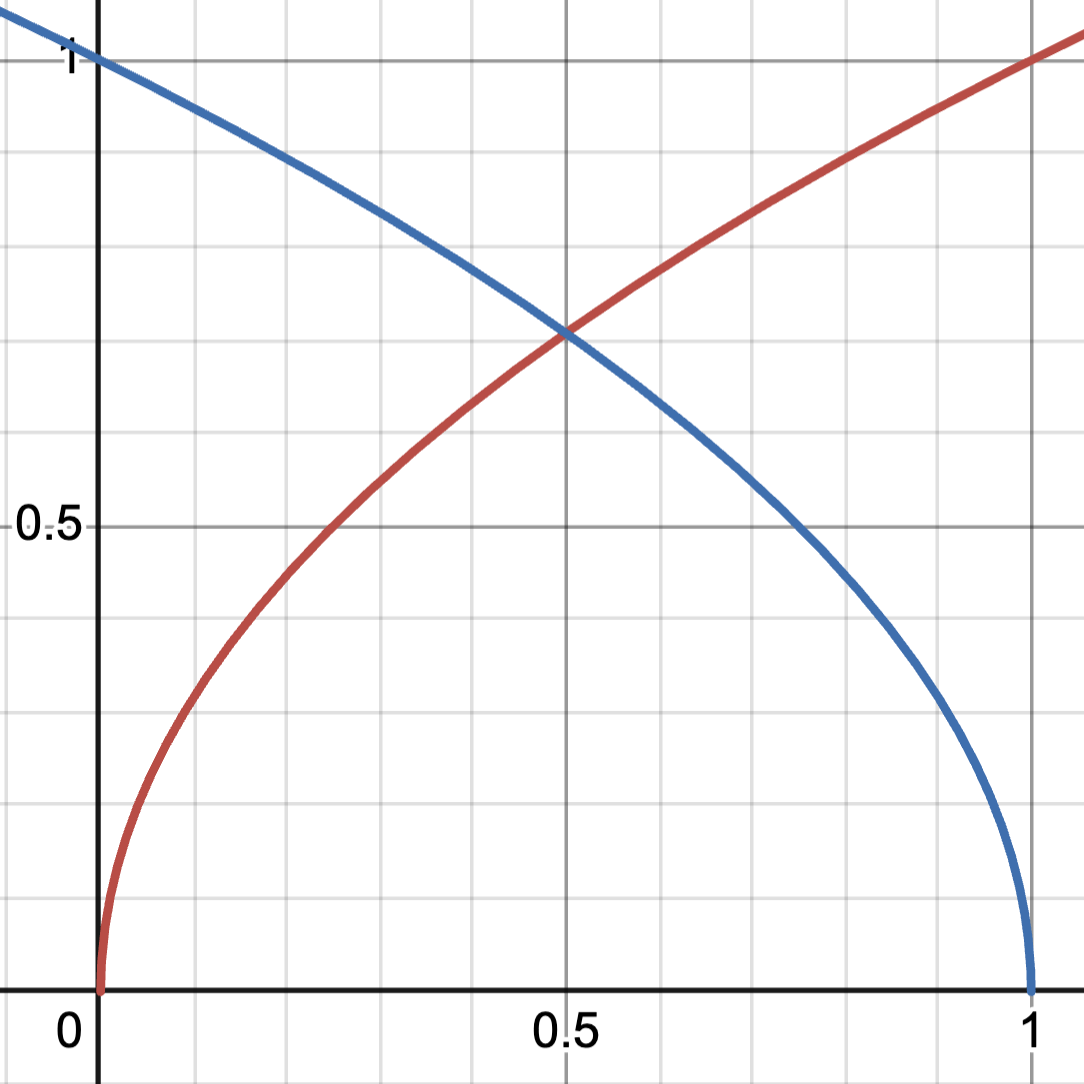
\includegraphics[width=0.9\linewidth]{images/beta_sqrtbeta}
	\label{fig:wrapfig}
\end{wrapfigure}

Cả hai đại lượng này thay đổi theo thời gian trong quá trình diffusion, từ đó quyết định mức độ ngẫu nhiên và mức độ giữ lại trạng thái trước đó qua từng bước. Chúng đóng vai trò quan trọng trong việc xác định cách thức mà trạng thái của hệ thống tiến dần đến một trạng thái cuối cùng hoặc trạng thái cân bằng.



%Praesent in sapien. Lorem ipsum dolor sit amet, consectetuer 
%adipiscing elit. Duis fringilla tristique neque. Sed interdum

%\begin{figure*}[p]
%	\centering
%	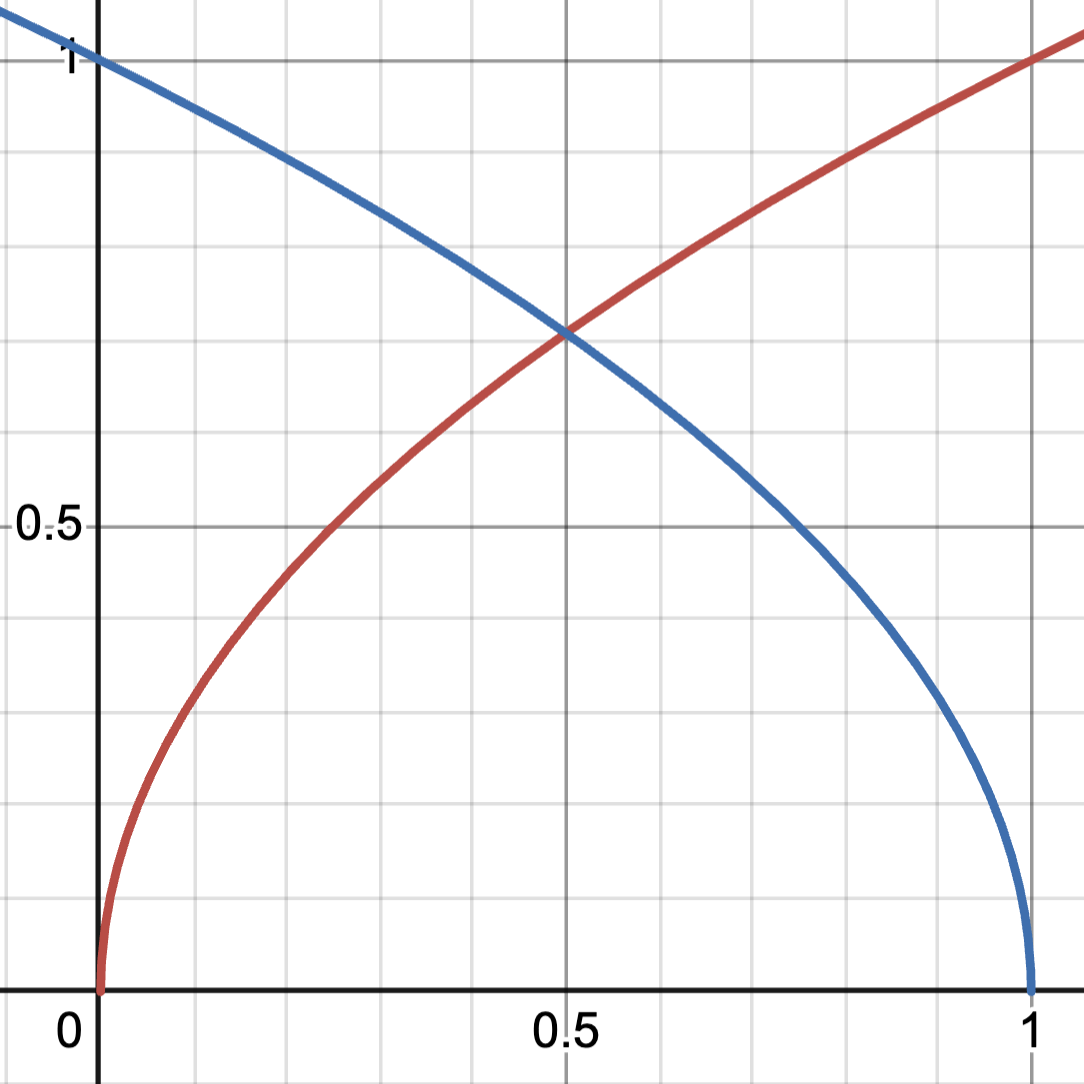
\includegraphics[width=0.5\linewidth]{images/beta_sqrtbeta}
%	\caption{Sự thay đổi của $\sqrt{\beta}$ và $\sqrt{1-\beta}$}
%	\label{fig:beta_sqrtbeta}
%\end{figure*}


%You can put more than one value in the parameter, for instance, if you write [ht] LaTeX will try to position the figure here, but if it's not possible (the space may be insufficient) then the figure will appear at the top of the page. It is recommended to use more than one positioning parameter to prevent unexpected results.
